\documentclass[11pt,letterpaper]{article}
\usepackage[spanish]{babel}
%\usepackage[ansinew]{inputenc}
\usepackage[utf8]{inputenc}
%\usepackage[latin1]{inputenc}
\usepackage[letterpaper,includeheadfoot, top=0.5cm, bottom=3.0cm, right=2.0cm, left=2.0cm]{geometry}
\renewcommand{\familydefault}{\sfdefault}

\usepackage{graphicx}
\usepackage{color}
\usepackage{hyperref}
\usepackage{amssymb}
\usepackage{url}
%\usepackage{pdfpages}
\usepackage{fancyhdr}
\usepackage{hyperref}
\usepackage{subfig}

\usepackage{listings} %Codigo
\lstset{language=C, tabsize=4,framexleftmargin=5mm,breaklines=true}

\begin{document}
% --------------- ---------PORTADA --------------------------------------------
\newpage
\pagestyle{fancy}
\fancyhf{}
%-------------------- CABECERA ---------------------
\fancyhead[L]{ 
\includegraphics[scale=0.9]{img/logo_die.pdf} }
%------------------ TÍTULO -----------------------
\vspace*{6cm}
\begin{center}
\Huge  {Informe Final} \\
\vspace{1cm}
\huge {EL6908 - Introducción al Trabajo de Título}\\
\vspace{1cm}
\huge {\textit{Diseño e Implementación del Software de Control para el Computador a Bordo de un Pico-Satélite}}\\
%\vspace{1cm}
%\small {Título pequeño} 
\end{center}
%----------------- NOMBRES ------------------------
\vfill
\begin{flushright}
\begin{tabular}{ll}
\textbf{Autor} &: Carlos González C.\\
\textbf{Profesor Guía} &: Marcos Díaz Q.\\
\textbf{Profesor EL6908} &: Jorge Lopez H.\\
& \today\\
& Santiago, Chile.
\end{tabular}
\end{flushright}

% ·············· ENCABEZADO ············
\newpage
\pagestyle{fancy}
\fancyhf{}
%\fancyhead[L]{\rightmark}
\fancyhead[L]{\small \rm \textit{Sección \rightmark}}
\fancyhead[R]{\small \rm \textbf{\thepage}}
\fancyfoot[L]{\small \rm \textit{Informe Final}}
\fancyfoot[R]{\small \rm \textit{EL6908 - Introducción al Trabajo de Título}}
%\fancyfoot[C]{\thepage}
\renewcommand{\sectionmark}[1]{\markright{\thesection.\ #1}}
\renewcommand{\headrulewidth}{0.5pt}
\renewcommand{\footrulewidth}{0.5pt}

% =============== INDICE ===============

\tableofcontents
\listoffigures
% \listoftables

% =============== IDENTIFICAION ===============
\newpage
\section{Identificación}

\subsection{Alumno}

\begin{itemize}
	\item \textbf{Nombre:} Carlos Eduardo González Cortés
	\item \textbf{Rut:} 17059374-k
	\item \textbf{Nº de matrícula:} 27004652
	\item \textbf{Dirección:} San Ignacio 999, Dpto 22C, Santiago, Chile
	\item \textbf{Celular:} 75535716
	\item \textbf{Correo:} carlgonz@ug.uchile.cl
\end{itemize}

\subsection{Profesor Guía}

\begin{itemize}
	\item \textbf{Nombre:} Marcos Díaz Quezada
	\item \textbf{Dirección:} Av. Tupper 2007, Of. 510, Santiago, Chile
	\item \textbf{Teléfono:} Fono: (56)-2-978-4204
	\item \textbf{Correo:} mdiazq@ing.uchile.cl
\end{itemize}

% =============== CUERPO ===============
\newpage
\section{Título del tema}

Diseño e implementación del software de control para el computador a bordo de un pico-satélite.

\section{Fundamentación y objetivos generales}

Esta memoria se enmarca en el desarrollo del proyecto SUCHAI que consiste en la implementación, lanzamiento y operación de un pico-satélite Cubesat, siendo esta la primera aproximación en esta materia para la universidad y el país. Uno de los componentes fundamentales de un satélite es su computador abordo, sistema encargado de dar inteligencia y operatividad al satélite durante todo su tiempo de vida útil en el espacio. En el caso de un pico-satélite se tiene el desafío de dotar de todas la funcionalidades estándar de un satélite en un sistema computacional de recursos extremadamente limitados, estamos hablando de sistemas embebidos que utilizan microcontroladores de baja potencia y capacidad de cómputo como microcontroladores PIC24 o PIC18.

El objetivo de este trabajo es el diseño, desarrollo e implementación del \textit{software} que gobierna el computador a bordo del satélite. Se requiere diseñar una arquitectura de \textit{software} que abarque desde controladores de hardware hasta la aplicación final para el control de satélite. Esta arquitectura debe cumplir con requerimientos de calidad de \textit{software} como modularidad, expansibilidad y facilidad de mantenimiento estando adaptada en específico a sistemas embebidos que emplean microcontroladores de gama media.

La implementación se llevará a cabo en específico para el satélite SUCHAI y busca proveer la funcionalidad básica de este sistema que incluye la interacción de un computador a bordo, un sistema de control de energía y un sistema de comunicaciones. De esta manera el \textit{software} de control se cuenta como un recurso más que será considerado y adaptado a la necesidades específicas del proyecto en la etapa de integración general de sistemas del satélite.

\section{Bibliografía y Estado del Arte}

Para el desarrollo del trabajo de título serán fundamental la siguiente bibliografía:
\begin{itemize}
	\item R. Barry, \textit{Using the FreeRTOS Real Time Kernel. A Practical Guide, PIC32 Edition.}, 1st ed., USA: Real Time Engineers, 2009.
	\item I. Sommerville, \textit{Software Engineering}, 9nd ed., USA: Addison-Wesley, 2011.
	\item S. Heat, \textit{Embedded Systems Design}, 2nd ed., England: Newnes, 2003.
	\item L. Di Jasio \textit{Programming 16-Bit PIC Microcontrollers in C} , 1st ed. USA: Elsevier, 2007.
\end{itemize}

Lo tópicos relacionados con el desarrollo de sistemas embebidos utilizando microcontroladores PIC y sistemas operativos de tiempo real como FreeRTOS se encuentran bastante desarrollados y bien documentados, en este sentido lo más interesante es tener una visión detallada del funcionamiento de un sistema embebido desde la perspectiva de arquitectura de hardware para un trabajo a muy bajo nivel. Esto se suma a la necesidad de utilizar herramientas de ingeniería de software para desarrollar una arquitectura que logre cumplir con los requerimientos de una misión crítica como la que corresponde al proyecto SUCHAI.\\

Por otro lado se encuentra el desarrolla de un sistema de control para un satélite, específicamente un satélite tipo Cubesat. Esta es un área totalmente nueva donde la mayoría de la información disponible no es formal y se basa en experiencias previas desarrolladas por otras unidades educativas en el extranjero. En la universidad de Chile y en el país no se han desarrollado proyectos similares hasta ahora, de modo que este trabajo sienta un precedente importante para futuras misiones aeroespaciales en la región, proyectos que tendrán una base bastante sólida sobre la cual comenzar.


\section{Objetivos específicos}
Los objetivos específicos del proyecto se enumeran a continuación

\begin{itemize}
 \item Diseñar una arquitectura de \textit{software} para el sistema de control del satélite
 \item Implementar controladores de hardware para el microcontrolador
 \item Implementar controladores de periféricos principales (Transceiver, EPS y RTC)
 \item Integrar un sistema operativo de tiempo real multitarea como sistema embebido 
 \item Implementar el flujo principal de la arquitectura del \textit{software} de control del satélite
 \item Integrar sistema de comunicaciones al \textit{software} de control
 \item Integrar sistema de energía al \textit{software} de control
 \item Pruebas del sistema integrado
\end{itemize}

El listado de objetivos presenta un orden temporal en la ejecución de estas tareas puesto que objetivo es dependiente del cumplimiento de los objetivos anteriores. El trabajo se puede considerar terminado cuando se ha probado la implementación e integración del \textit{software} con los módulos de comunicaciones y energía obteniendo un sistema satelital con las mínimas funcionalidades.

\section{Antecedentes generales}

El trabajo de memoria se enmarca en el proyecto SUCHAI (Satellite of University of Chile for Aerospace Investigation) cuyo objetivo es desarrollo, lanzamiento y operación de un pico-satélite tipo Cubesat con fines educacionales y de investigación. El proyecto es generado por el profesor guía quien convoca a alumnos de pregrado a desarrollar el proyecto bajo la guía del líder del proyecto el Ing. Alex Becerra.\\

El éxito del proyecto depende del correcto desarrollo e integración de tres áreas fundamentales de cualquier vehículo satelital: la inteligencia programada en el computador a bordo; el suministro y gestión de la energía eléctrica mediantes paneles solares y baterías; y la capacidad de contar con un enlace de radio que permita obtener información de telemetría del satélite así como enviar telecomandos que definan su operación.\\

Contar con un vehículo espacial de estas características permite a los académicos de diferentes áreas el desarrollo de experimentos y estudios que requieren condiciones especiales de gravedad; atmosféricas; o una determinada altitud. En este caso se pretende poner en órbita como payloads: una dispositivo \textit{lagmuir probe} que estudia variaciones del plasma en la ionosfera; un experimento del departamento de física sobre electrónica en gravedad cero; así como una cámara fotográfica para captar la tierra y el satélite mismo. 

\section{Antecedentes específicos}

El proyecto se encuentra en considerable estado de avance, pero este trabajo de memoria pretende formalizar; formar metodología; y documentar técnicas de desarrollo de software para sistemas electrónicos de muy bajo nivel para misiones críticas como lo significa una misión aeroespacial.\\

No obstante el proyecto comienza desde cero, debido a que el conocimiento sobre desarrollo de proyectos aeroespaciales en la universidad y en el país se encontraba completamente detenido.

\section{Infraestructura disponible}
\subsection{Instalaciones}
El proyecto se desarrolla en las dependencias de la facultad, específicamente el laboratorio SPEL (\textit{Spacial and Planetary Exploration Laboratory}), tercer piso del edificio de Electrotecnologías. Este laboratorio alberga proyectos relacionados el desarrollo de radiosondas para monitoreo de condiciones climáticas, radares y proyectos aeroespaciales como el SUCHAI.

\subsection{Hardware}
\paragraph{Cubesat Kit:}
Parte fundamental del hardware disponible corresponde a un Cubesat Kit adquirido a la compañía Pumpkins. El kit incluye la estructura de un Cubesat de una unidad con un microcontrolador PIC24F256GA110; una placa de desarrollo para el mismo sistema; y herramientas de programación y \textit{debug} para el microcontrolador.

%···················· FIGURE ····················
\begin{figure}[!h] 
\centering 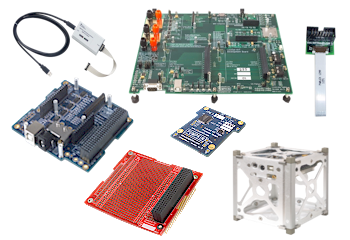
\includegraphics[scale=0.8]{img/cubesatkit.jpg}
\caption{Cubesat Kit} \label{cubesatkit}
\end{figure}
%················································

\paragraph{Transceiver:}
Se cuenta con un sistema de comunicaciones que consta de un \textit{transceiver} satelital FSK para la banda de 430MHz de la empresa ALLSPACE adaptado al estándar Cubesat. Es el sistema encargado de recibir los telecomandos desde tierra y transmitir hacia la estación terrena la telemetría generada por el satélite.\\

Se cuenta además con una estación terrena dotada con un sistema de radio en la banda de 430MHz, incluyendo antena y control de posición de la misma; un TNC para digitalizar la señal de radio; y un servidor para controlar los equipos de forma remota.

\paragraph{Sistema de gestión de energía:}
Se adquiere un sistema de control de energía para el satélite que incluye baterías de litio, panales solares y un sistema de control para medir variables importantes de energía y ajustar su funcionamiento.

\paragraph{Equipos de medición}
El laboratorio cuenta con un osciloscopios; analizadores de espectro; generadores de señales; cajas limpias, para pruebas que requieren entornos descontaminados; entre otros.

\subsection{Software}
La mayor parte del software utilizado por el proyecto es de código libre o gratuito. Se desataca la amplia utilización de sistemas Linux para el desarrollo de este trabajo.

\paragraph{Entorno de desarrollo:}
Para el desarrollo de la aplicación para el microcontrolador PIC24F se utiliza el entorno de desarrollo MPLABX de Microchip, que es gratuita y se observa en la figura \ref{mplabx}; se utiliza el compilador MPLAB C30, en versión lite, gratuito; se tiene un sistema de control de versiones mediante SVN.

%···················· FIGURE ····················
\begin{figure}[!h] 
\centering 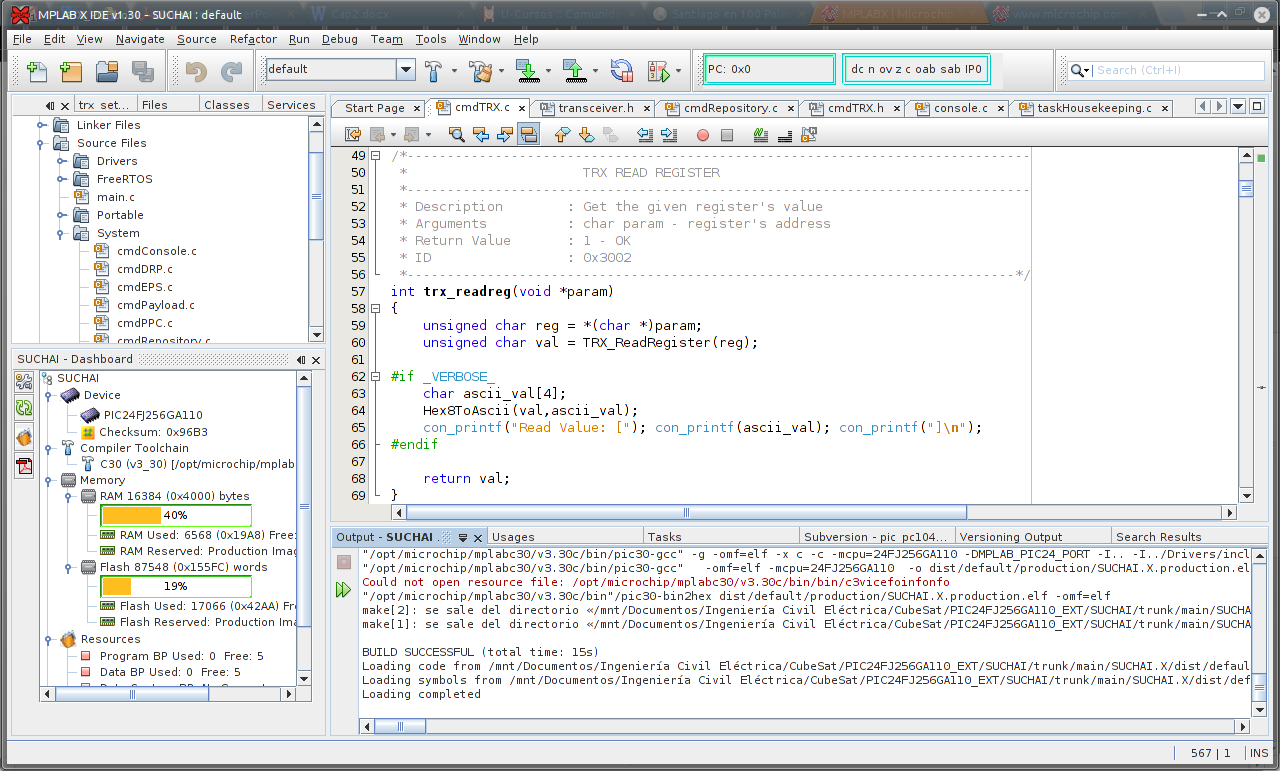
\includegraphics[scale=0.4]{img/mplabx.png}
\caption{Entorno de desarrollo MPLABX} \label{mplabx}
\end{figure}
%················································

\paragraph{Sistema operativo:}
Para dotar de funcionalidades avanzadas de multitarea al microcontrolador se ha utilizado el sistema operativo de tiempo real FreeRTOS de código libre y gratuito; adaptado especialmente a microcontroladores de gama media como el utilizado en el proyecto.

\section{Condiciones contractuales}
El desarrollo de este trabajo se enmarca dentro del proyecto SUCHAI el cual es patrocinado y financiado por la Facultad de Ciencias Físicas y Matemáticas de la Universidad de Chile.

Siendo alumno regular de la carrera Ingeniería Civil Electricista de la Universidad de Chile, parte del trabajo realizado para esta memoria ha sido considerado en el desarrollo de los cursos Seminario de Diseño e Innovación Tecnológica I, II y III (ME4030, EL5030, EL6030).


% % ============= BIBLIOGRAFIA ==============
% \newpage
% \begin{thebibliography}{5}
% 	\bibitem{cmos} R. Jacob Baker, \textit{CMOS. Circuit Design, Layout, and Simulation}, 2nd ed., USA: IEEE Press, 2005
% 	
% \end{thebibliography}

\end{document}

% % ················ IMAGEN ·················
% \begin{figure}[ht!]
% \centering
% \fbox{\includegraphics[scale=0.6]{img/flujo.png}}
% \caption{Flujo de caja anual}\label{flujo}
% \end{figure}
% %··········································

% % ················ IMAGEN ·················
% \begin{figure}[ht!] \centering
% \subfloat[Esquemático]{\includegraphics[scale=0.44]{img/seguidor.png}}
% \subfloat[Simulación]{\includegraphics[scale=0.45]{img/seguidor1.png}}
% \caption{Simulación como seguidor de voltaje}\label{seguidor}
% \end{figure}
% %··········································